%! Author = magnus.silverdal
%! Date = 2020-11-20

% Preamble
\documentclass[11pt]{beamer}

% Packages
\usepackage{amsmath}
\usepackage{pgfplots}
\usetheme{Copenhagen}
\title{Newton Raphsons metod för att lösa ekvationer}
\author{Magnus Silverdal}
\institute{NTI Gymnasiet}
\date{\today}

% Document
\begin{document}
    \frame{\titlepage}
    \begin{frame}
        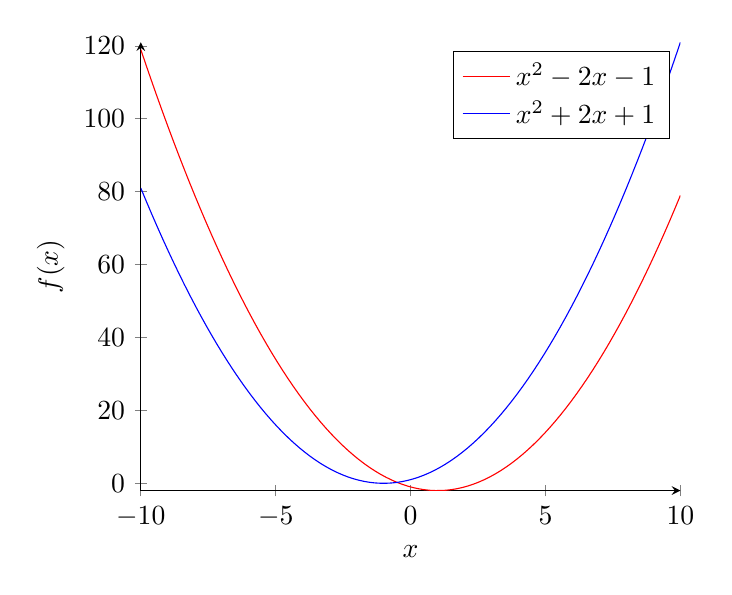
\begin{tikzpicture}
            \begin{axis}[
            axis lines = left,
            xlabel = $x$,
            ylabel = {$f(x)$},
            ]
%Below the red parabola is defined
                \addplot [
                domain=-10:10,
                samples=100,
                color=red,
                ]
                {x^2 - 2*x - 1};
                \addlegendentry{$x^2 - 2x - 1$}
%Here the blue parabloa is defined
                \addplot [
                domain=-10:10,
                samples=100,
                color=blue,
                ]
                {x^2 + 2*x + 1};
                \addlegendentry{$x^2 + 2x + 1$}

            \end{axis}
        \end{tikzpicture}
    \end{frame}
    \begin{frame}
        \frametitle{Exempel 1}

%Here begins the 3d plot
        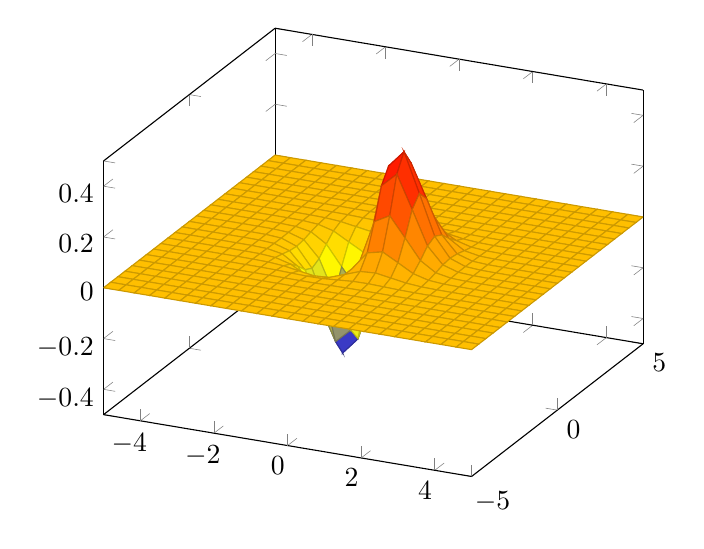
\begin{tikzpicture}
            \begin{axis}
                \addplot3[
                surf,
                ]
                {exp(-x^2-y^2)*x};
            \end{axis}
        \end{tikzpicture}
        \end{frame}
    \begin{frame}
        \begin{tikzpicture}
            \GraphInit[vstyle=Welsh]
            \SetGraphUnit{2}
            \Vertices{circle}{A,B,C,D,E}
            \SetUpEdge[style={->}]
            \Edges[label=1](A,B)
            \Edges[label=1](B,C)
            \Edges[label=1](C,D)
            \Edges[label=$1$](D,E)
            \Edges[label=x1](A,C)
            \Edges[label=x2](A,D)
            \Edges[label=x3](A,E)
            \SetVertexNoLabel
        \end{tikzpicture}
    \end{frame}


\end{document}